\justifying

%%%%%%%%%%%%%%%%%%%%%%%%%%%%%%%%%%%%%%%%%%%%%%%%%%
\section{Introduction} \label{sec:intro}
%%%%%%%%%%%%%%%%%%%%%%%%%%%%%%%%%%%%%%%%%%%%%%%%%%

Solar flares are the largest magnetic events in our solar system. They are characterized by the eruptive release of magnetic energy, and manifest as localized transient heating of coronal plasma to temperatures over $\sim$ 10~MK. Flares are characterized by the full-disk integrated peak soft X-ray flux observed by the X-Ray Sensor onboard the {\it Geostationary Operational Environmental Satellites} \citep[{\it GOES}/XRS,][]{xrs} (``\textit{GOES class}''). The various components of the flare manifest in different wavelengths of the electromagnetic spectrum. The flare arcade and the fan exhibit the thermal plasma, while the majority of the non-thermal energy is from the foot points \citep{benz17}. The hot coronal plasma exhibited by flares is generally attributed to chromospheric evaporation, heated by the collisions of the flare-accelerated electrons in the impulsive phase \citep{fletcher11}. There is also strong evidence that the plasma might be directly heated in the corona in some cases \citep[e.g.][]{longcope11, reeves17}. 

There have been several works \citep{stosire07,emslie12,inglis14,warmuth16a,warmuth16b,ash17} that study the partition between the thermal and non-thermal energies in flares, which holds key insight into the relevant underlying physical processes in the flares. The results have been contradictory, and there is no consensus on whether non-thermal energetic electrons have enough energy to power the observed thermal energy component of smaller flares. These studies usually use peak thermal energy as a representative of the bulk thermal output of the flares. While these quantities are fair representation of the bulk thermal output of the flare, identifying subtle differences in the heating mechanisms at play at different stages of the flares requires a quantification of the thermal energy as a function of time.

There are several studies \citep{hilarie05,caspi10} that estimate thermal energy as a function of time. The thermal energy of the flares is defined as 
\begin{equation}
\mathrm{U_{Th}~\simeq~3n_{e}k_{B}TV}f,
\end{equation} \label{eq:t_eneg_1}
 where `$\mathrm{n_{e}}$' is the electron number density of the flaring plasma, `V' is the volume of the flaring plasma, `\textit{f}' is the volume filling factor, and `T' is the instantaneous temperature. One of the key challenges in characterizing the flares' thermal energy is determining the volume. 

\cite{li23} used $\frac{1}{e^{2}}$ contour of soft X-ray emitting region to identify the flare area `A', which was subsequently used to estimate the volume, $V\sim A^{\frac{3}{2}}$. \cite{zhang19} used a similar method, using intensity threshold on AIA 131~{\AA} observation, to estimate the flare area (A). \cite{hilarie05} used a similar method with {\it Reuven Ramaty High Energy Solar Spectroscopic Imager} \citep[{\it RHESSI},][]{rhessi} soft X-ray images to estimate the lower limit of the volume. They used {\it RHESSI} hard X-ray imaging to estimate the distance between two footpoints. Assuming a perfect ``arc-shaped" loop they calculated the upper estimate of the volume and concluded that the largest source of uncertainty in determining the thermal energy arises from the uncertainty in the filling factors.

\cite{hilarie05} also estimated the evolution of cumulative non-thermal energy injected by the electrons by assuming a thick-target model \citep{brown71} and fitting the {\it RHESSI} spectrum of the events. They fitted the {\it RHESSI} spectra in 25{--}35 keV bands to determine the non-thermal energies in time bins with significant emission above 25 keV. This process ensures a better accuracy for determining non-thermal energy by dividing the flare into short time intervals with large energy inputs, resulting in small thermal energy losses. They found that the non-thermal cumulative energy was larger than the thermal component of the flare for most of the duration of the flare. This is expected as radiative cooling significantly lower the temperature of the flare arcade as the flare evolves. They also deduced that during the early impulsive phase, the cumulative non-thermal energy could be lower than the thermal energy, depending on the estimates used for the flaring plasma volume. 

The filling factor `\textit{f}' quantifies the fraction of the apparent volume that is filled with the plasma of a specific temperature. It might also hold information about the geometric projection effects of the real volume into the apparent projected volume that is observed. Due to the highly multi-thermal nature of the flaring plasma and rapidly changing volume during the rise phase of the flare, it is challenging to define a filling factor that describes the plasma volume across the evolution of the flare. %Furthermore, most of the statistical studies so far, deals with bolometric or time averaged quantities near the peak of the flare.}
%This would indicate that direct heating possibly happens before or during the impulsive phase of flares.

\cite{caspi10} studied super hot flares from {\it RHESSI} observations, and used a 50\% intensity contour of cleaned {\it RHESSI} images to estimate the flare area, A. The volume $V=\frac{4}{3}\pi (A/\pi)^{3/2}$ was inferred from the area assuming spherical symmetry.  The two temperature components from the {\it RHESSI} spectral fit were assigned a volume V/2 each to estimate the total thermal energy. In all of these cases, the assumption of symmetrical expansion is useful because the thermal energy was estimated from a spectra obtained by integrating multiple pixels. There is no reliable way to address the spatially varying multi-thermal nature of the flaring plasma in these cases. 

In addition to the bulk thermal plasma in the flare loop, there are studies that suggested completely different heating mechanisms at play in specific flares. For example, \citet{longcope11} suggested a super hot plasma component in flares is directly heated in the corona in some large solar flares. Sustained temperatures in supra-arcade fans in flares have been hypothesized to be caused by supra-arcade down flows \citep[e.g.][]{reeves17}, suppression of conduction by turbulence \citep[e.g.][]{xie23} or global compression from reconnection inflows \citep[e.g.][]{reeves19}. These processes are distinctly different from chromospheric evaporation, which is characterized by the development of the hard X-ray foot-points and increasing intensity of soft X-ray and EUV-emitting plasma as the loops fill up.

%%%%######%%%%%%
\begin{figure}[ht!]
    \centering
    \includegraphics[trim={0cm 0.5cm 1.2cm 0.5cm},clip,width=\textwidth]{flare_pos.pdf}
    \caption[Position of various instruments during the flares.]{Position of various instruments during the flares. AIA 193~{\AA} observations during 2021 Oct 28 (panel a) and EUVI 171~{\AA} observation during 2020 Nov 29 (panel c) in Heliographic Stonyhurst (HGS) coordinates. The two flares studied here are enclosed by white dotted circle. The projected positions of {\it Solar Orbiter}, {\it SDO} and {\it STEREO-A} are marked as labelled. Positions of various spacecrafts projected onto the Heliocentric Inertial (HCI) frame for the for 2021 Oct 28 (panel c) and 2020 Nov 29 (panel d), as labelled.}
    \label{fig:sc_pos}
\end{figure}
%%%%######%%%%%%

Here we study the evolution of the thermal energy of two flares, \textit{viz.} M-class and X-class. We use existing tools and observations of the same region on the Sun from different vantages to estimate the volume of the flaring plasma more accurately. We show that a better estimate of the plasma volume affects the estimate of the thermal energy and has implications towards the energy budget of the flare. We also estimate the cumulative non-thermal energy deposited by the non-thermal electrons and compare it with our thermal energy estimates for the flare observed on 28 October, 2021. In \S\ref{sec:obs} we discuss the observations used in this {\bf chapter} and details of our analysis. We discuss our method for estimating the thermal energy in \S\ref{sec:therm}. In \S\ref{sec:los} and \S\ref{sec:non-therm}, we describe our method of volume estimation and cumulative non-thermal energy estimation, respectively. We discuss the results in \S\ref{res}.

%%%%%%
\begin{table}
    \centering
    \resizebox{\textwidth}{!}{%
    \begin{tabular}{||c|c|c||}
    \hline
    Instruments & Details & Flares\\
    \hline 
    \hline
      & 0.6 \arcsec/pix. Used&   \\
     {\it SDO}/AIA &  for estimating the thermal & 28 October, 2021 \\
     & properties. Temperature coverage & \& 29 November, 2020 \\
     & 5 $< log\ (T) <$ 7.5 & \\
         \hline
        & 2.5 \arcsec/pix. Has & \\
       & similar temp. response as AIA. & 28 October 2021 \\
      {\it GOES}/SUVI & Used for replacing saturated & \& 29 November, 2020 \\
       & AIA frames in DEM estimation & \\
       \hline 
        & 1 \arcsec/pix. Used simultaneously & \\
       & with AIA data in estimation of the thermal  & \\
     {\it Hindoe}/XRT  & properties. Temperature coverage  & 29 November, 2020 \\
       & 6.1 $< log\ (T) <$ 7.5, provides better & \\
       & constraints on the higher temp. end. & \\
       \hline 
       & 1.6 \arcsec/pix. Used & \\
       & for estimating the geometry & 28 October 2021  \\
     {\it STEREO-A}/EUVI   & of the arcade. 171 and 195 \AA & \& 29 November, 2020 \\
       & Observations are used with & \\
       & AIA 171 and 193 \AA. & \\
       \hline
        & X-ray imaging and spectroscopy in the  &   \\
       & 4-150 keV range. Soft X-ray imaging used & \\
      {\it SO}/STIX & for calculating the area of the flare. & 28 October 2021 \\
       &  Spectra used for constraining the thermal & \\
       & and non-thermal properties & \\
       \hline
       & Continuous full disk integrated soft X-ray light curve. & 28 October, 2021 \\
     {\it GOES}/XRS  & Used for estimating the bulk thermal & \& 29 November, 2020 \\
       & properties of the flare. & \\
       \hline
    \end{tabular}}
    \caption{List of the various instruments with their relevant specifications that were used for the analysis of the specific flares.}
    \label{tab:data}
\end{table}
%%%%%%


%%%%%%%%%%%%%%%%%%%%%%%%%%%%%%%%%%%%%%%%%%%%%%%%%%
\section{Observations and Data Analysis}\label{sec:obs}
%%%%%%%%%%%%%%%%%%%%%%%%%%%%%%%%%%%%%%%%%%%%%%%%%%

We study the two flares observed on 28 October, 2021 (X-class) and 29 November, 2020 (M-class) observed on the disk center and limb of the Sun, respectively, from the perspective of Atmospheric Imaging Assembly onboard the {\it Solar Dynamic Observatory} \citep[{\it SDO}/AIA,][]{sdo,aia} vantage point. For this study, we primarily use the observations from AIA, the Extreme Ultraviolet Imager onboard {\it Solar Terrestrial Relations Observatory-A} \citep[{\it STEREO-A}/EUVI,][]{stereo,euvi} and the Solar Ultraviolet Imager onboard {\it GOES} \citep[{\it GOES}/SUVI,][]{suvi}, along with imaging from the Spectrometer/Telescope for Imaging X-rays onboard {\it Solar Orbiter} \citep[{\it SO}/STIX,][]{so,stix,stix1}, the X-Ray Telescope onboard {\it Hinode} \citep[{\it Hinode}/XRT,][]{xrt} and the X-Ray Sensor onboard {\it GOES} \citep[{\it GOES}/XRS,][]{xrs}. For the relevant specification of the instruments used, refer to Table~\ref{tab:data}.

The positions of various spacecraft with respect to the flares' location on the solar disk is illustrated in Fig.~\ref{fig:sc_pos}. The AIA 193 {\AA} observation of the 2021 Oct 28 flare is projected to Heliographic Stonyhurst (HGS) coordinates in panel a, with {\it SDO} (magenta cross), {\it SO} (cyan circle) and {\it STEREO-A} (green triangle) positions marked with respect to the flare location in Fig.~\ref{fig:sc_pos}.a. The flare is marked with white dotted circle. The relative separation between the spacecrafts show the difference in the polar angle (vertical axis in Fig.~\ref{fig:sc_pos}.a) and azimuthal angle (horizontal axis in Fig.~\ref{fig:sc_pos}.a) introduced due to difference in vantages. The positions of the spacecrafts projected onto the Heliocentric Intertial (HCI) frame for the 2021 Oct 28 event is plotted in Fig.~\ref{fig:sc_pos}.b. The relative separation between the spacecrafts show the difference in azimuthal angle and the distance from the sun (distance from the center radially outwards in Fig.~\ref{fig:sc_pos}.b). We show the same for the 2021 Nov 29 flare in Fig.~\ref{fig:sc_pos}.c and d, with {\it STEREO-A}/EUVI 171 {\AA} emission projected to HGS and HCI coordinates.% {\bf We list out the various instruments used for the analysis of the two flares in Tab.~\ref{tab:data}.}

%%%%%%%%%%%%%%%%%%%%%%%%%%%%%%%%%%%%%%%%%%%%%%%%%%
\subsection{X flare on 28th October, 2021}\label{sec:x1-obs}
%%%%%%%%%%%%%%%%%%%%%%%%%%%%%%%%%%%%%%%%%%%%%%%%%%
%%--------------------------
\begin{figure}[ht!]
    %\hspace{-1cm}
    \centering
    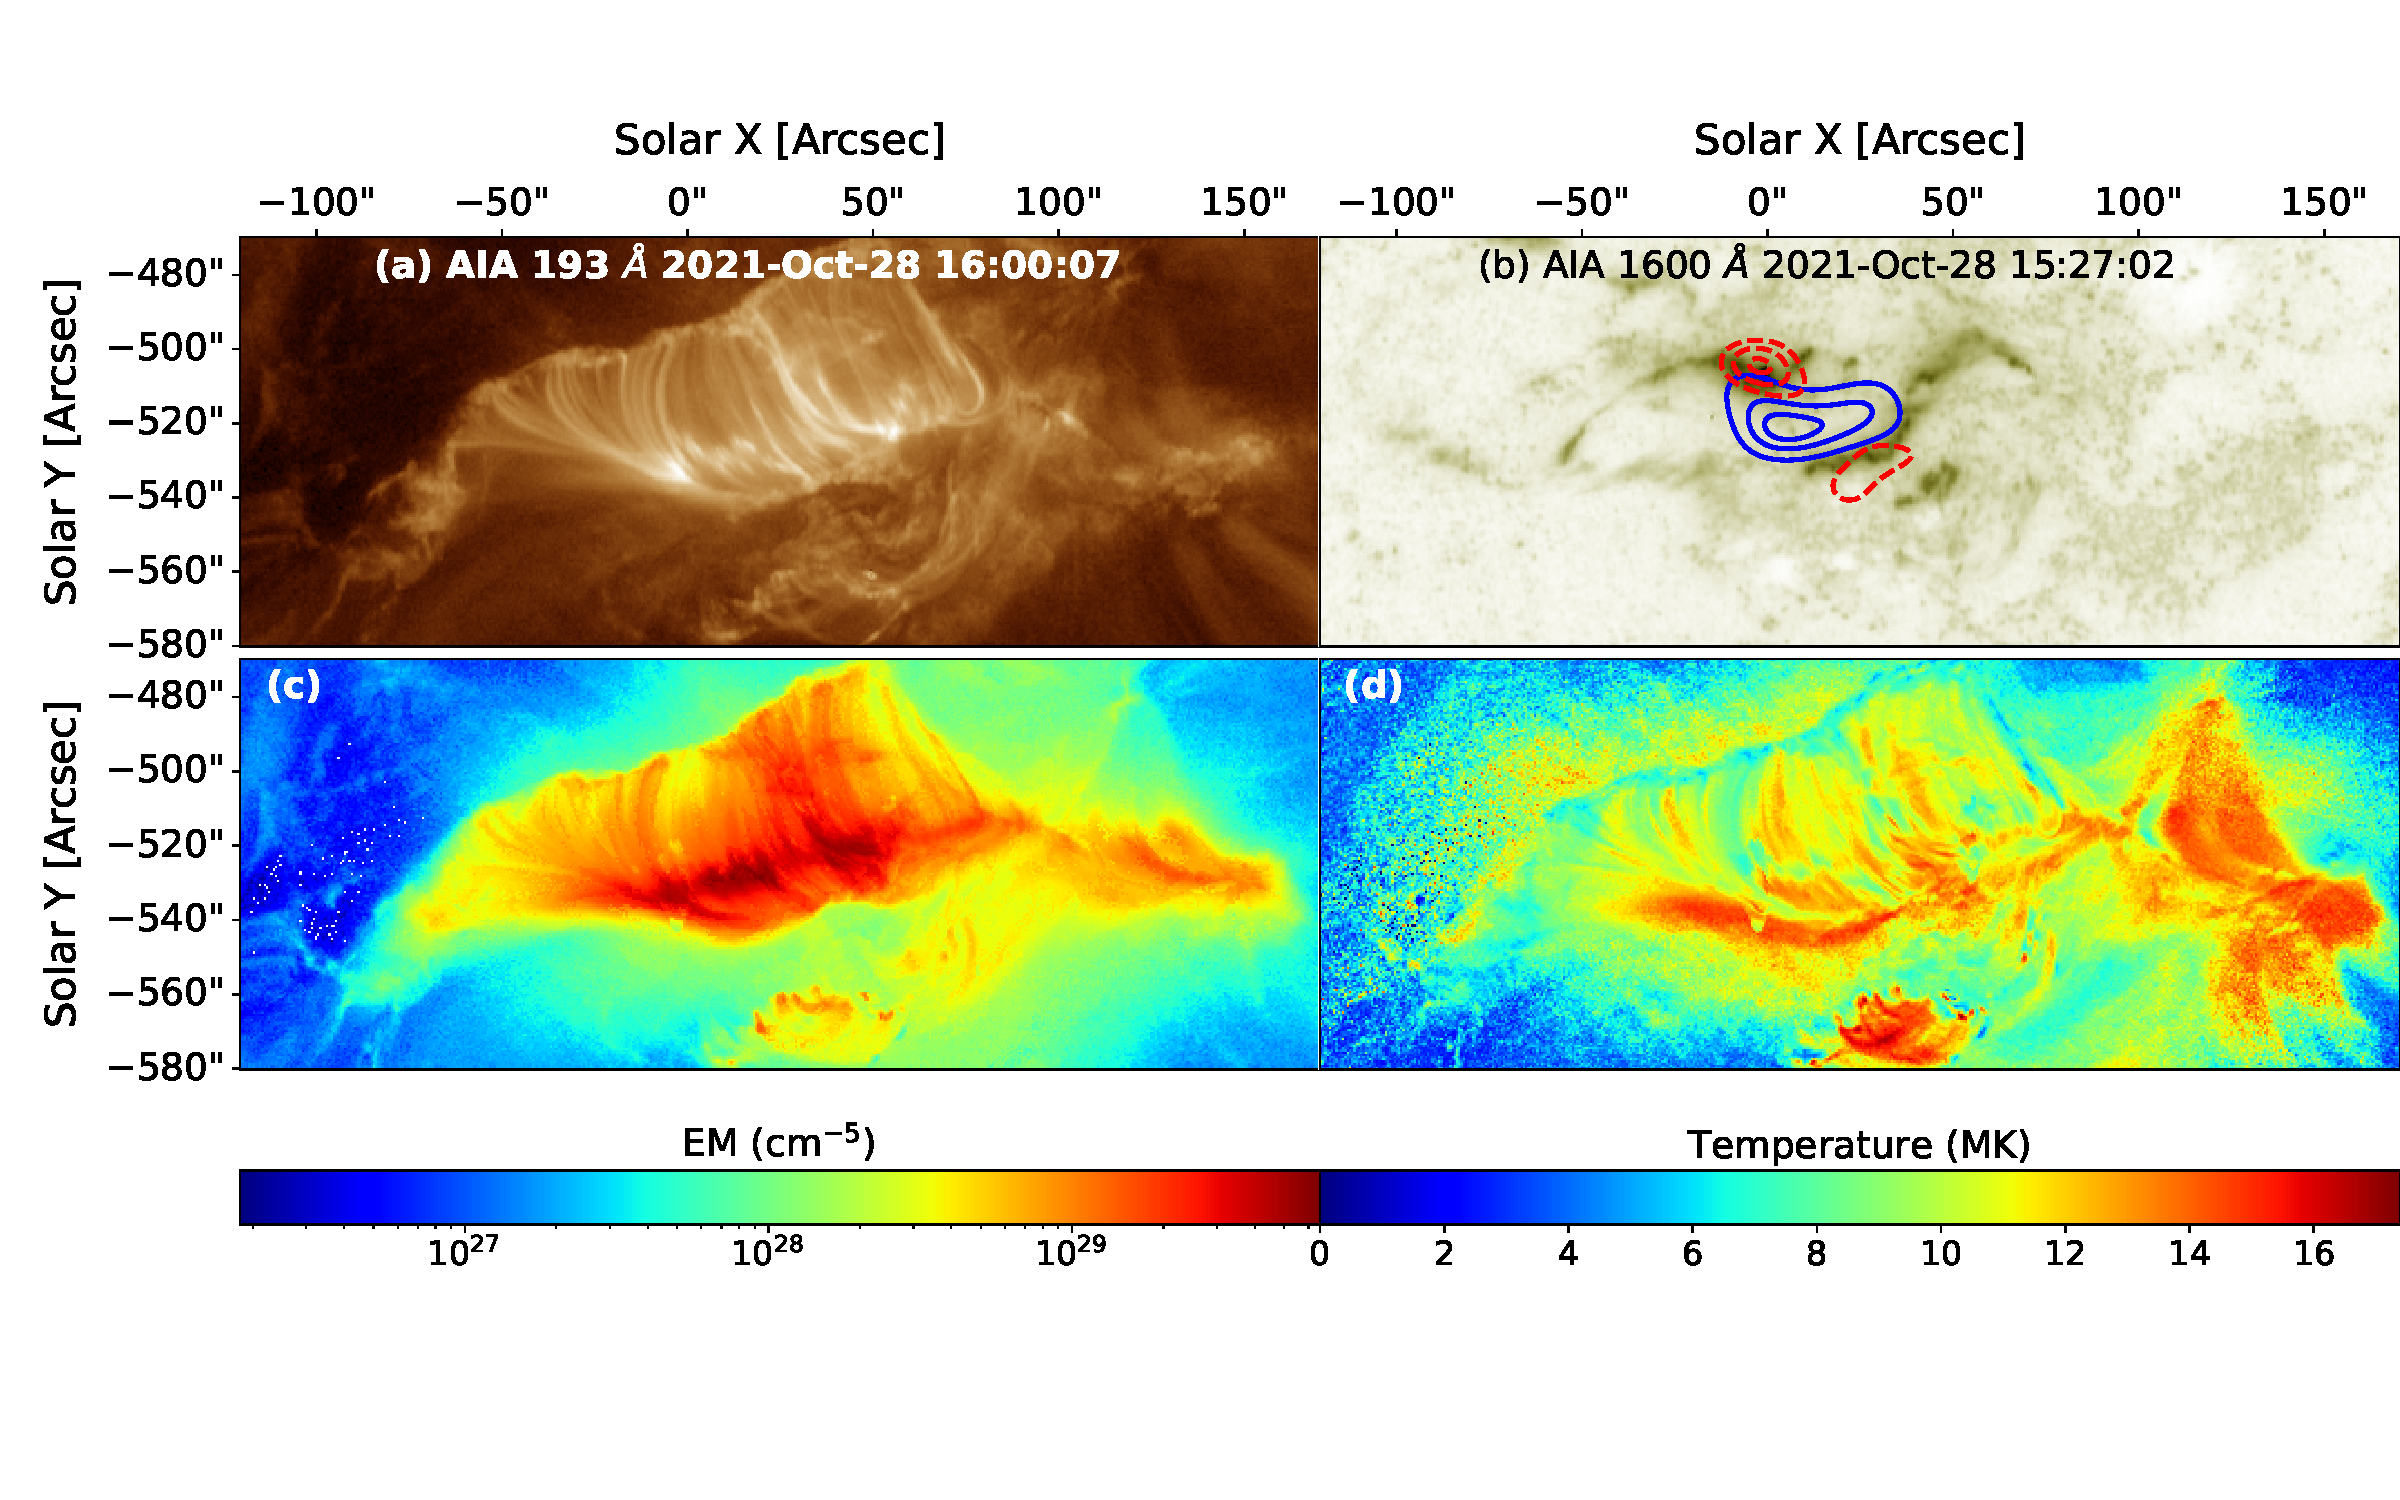
\includegraphics[width=0.95\textwidth,trim={0.3cm 4cm 0cm 2cm},clip]{oct28_align_new.pdf}
    \caption[Observation of the X-class flare on October 28, 2021.]{X-class flare observed on October 28, 2021. Panel (a): the post eruption arcade as observed in AIA 193~{\AA}. Panel (b): Two ribbon of the flare observed in AIA 1600 {\AA}, overplotted with STIX soft X-ray contours of 4{--}15 keV (solid blue lines) and hard X-ray contours of 15{--}25 keV (dashed red lines). Panel (c): the emission measure map of the region integrated over the temperature range of 5$<\log\,T<$7.4. Panel (d): the obtained DEM weighted temperature.}
    \label{fig:flare}
\end{figure}
%%--------------------------
The X1 flare occurred on Oct 28, 2021 (SOL2021-10-28T15:35) near $\sim~[0\arcsec,-500\arcsec]$ solar coordinates as seen from AIA. The flare was observed by {\it SDO}/AIA, {\it STEREO-A}/EUVI, {\it GOES}/SUVI, and XRT, along with {\it GOES}/XRS and STIX observations. AIA observations provide imaging with 94, 131, 193, 171, 211 and 335 {\AA} passbands. SUVI provides imaging with similar wavelengths as AIA: 94, 131, 195, 171, 195 and 284 {\AA}, while {\it STEREO-A}/EUVI provides imaging in 171, 195, 284 {\AA} coronal passbands. The flare exhibits a standard two-ribbon structure, along with a ridge at the top of the rising flare arcade \citep{longcope22}. The ridge most prominently shows up in the AIA 193 {\AA} channel with contributions from \ion{Fe}{12} and \ion{Fe}{24}. %\cite{longcope22} showed that the ridge was mainly created by the hotter \ion{Fe}{24} line (T~$\simeq$~17~MK) and a height of the flare arcade, $h~\simeq~20~Mm$. We use this ridge to identify the loop-top in the AIA observation and calculate the height of the loop (see \S\ref{sec:los} for further details).

{\it SO}/STIX provides X-ray imaging and spectroscopy in the 4-150 keV range. Spectroscopic observations are provided with 32 pre-defined energy channels distributed in this energy range. STIX is an indirect imager measuring visibilities in the Fourier space, and images can be reconstructed from these visibilities with different algorithms. We use the MEM-GE algorithm \citep{massa20} to construct the STIX intensity maps.

In Figure.~\ref{fig:flare} (top row) we display the flare as observed with AIA~193 {\AA} (panel a) and 1600~{\AA} (panel b, inverted colors). These images reveal the two ribbon nature of the flare with post eruption arcades \cite[see e.g.][]{TriBC_2004}. We also overplot the STIX intensity contours (15:27:40 {--} 15:28:00 UT) in 4{--}15 keV (blue solid lines) and 15{--}25 keV (red dashed lines), on an AIA 1600 {\AA} image during the rise phase of the flare (see Fig.~\ref{fig:flare}.b). The STIX hard X-ray contour aligns with AIA 1600 {\AA} ribbons.


%%--------------------------
\begin{figure}[ht!]
\centering
    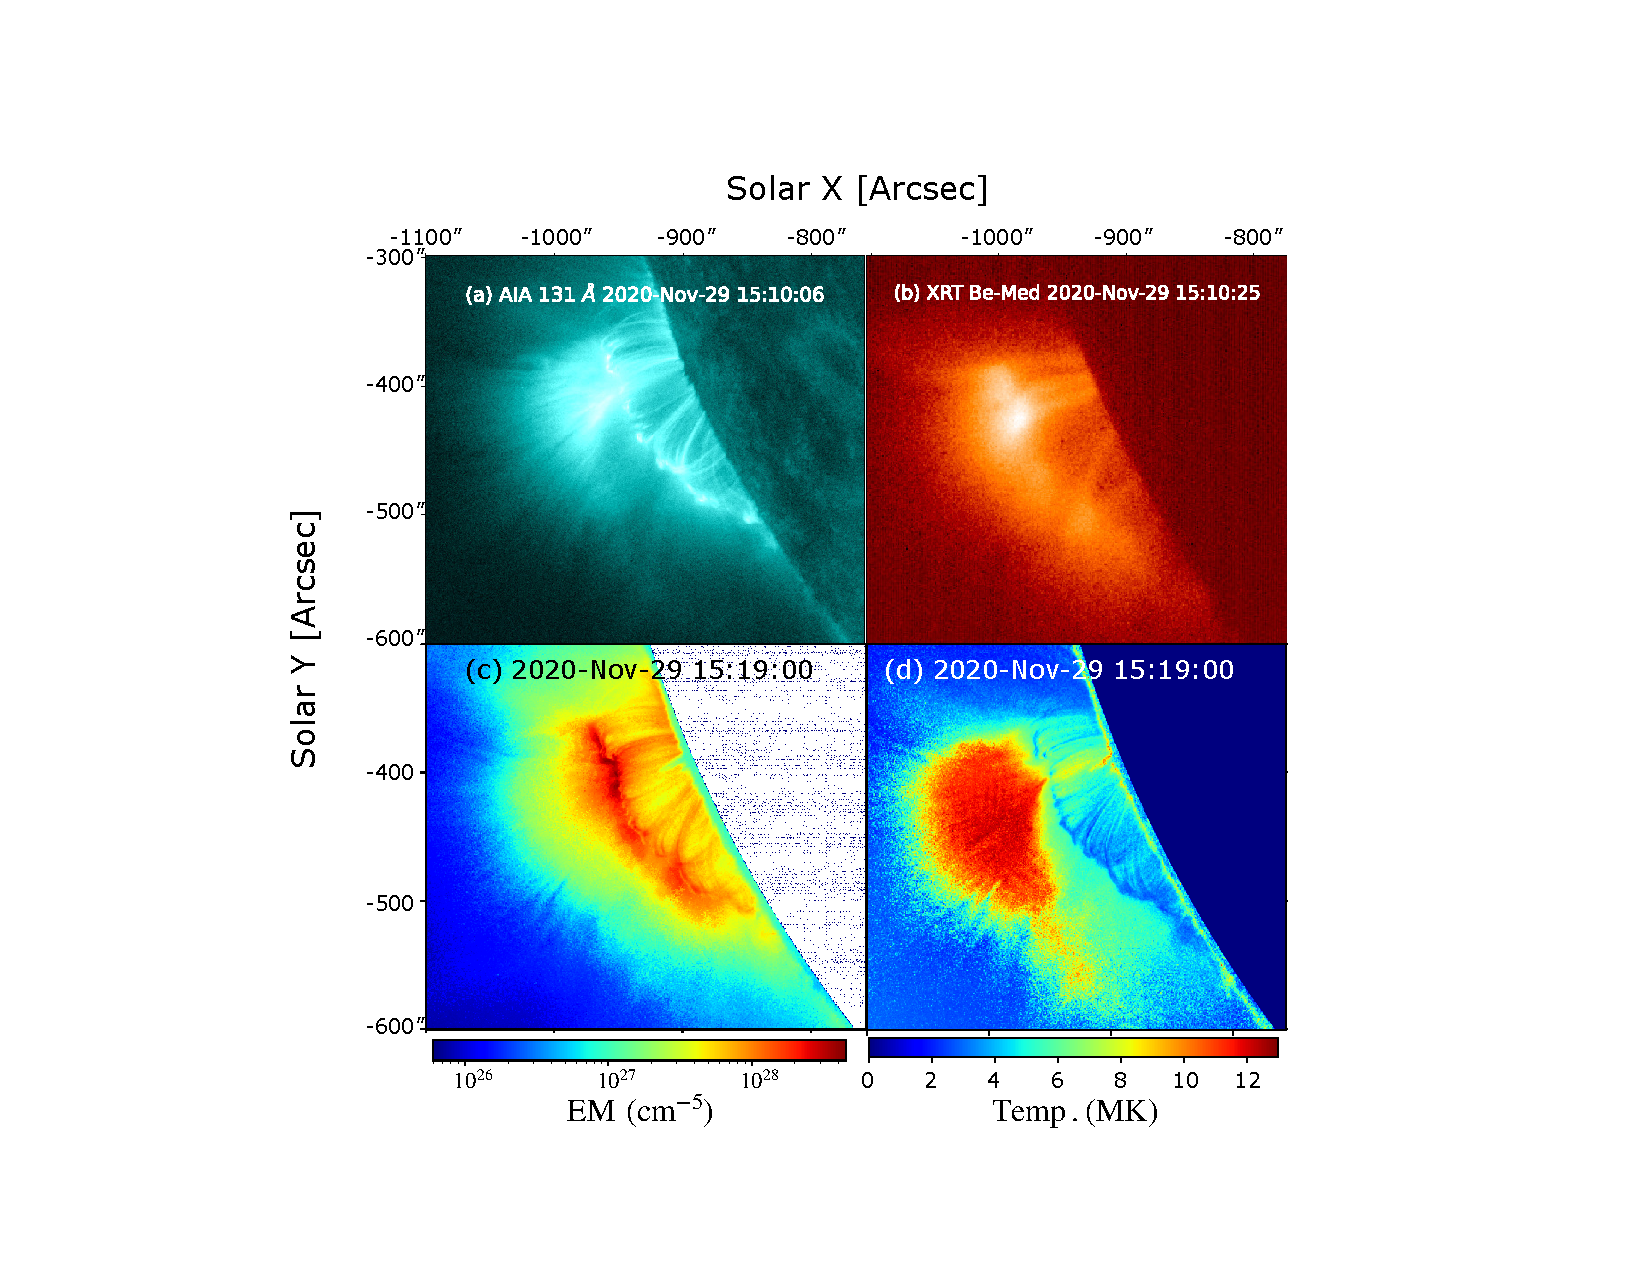
\includegraphics[trim={4.8cm 2.5cm 6cm 2.5cm},clip,width=0.8\textwidth]{nov_29_align.pdf}
    \caption[Observation of the M-class flare on November 29, 2020.]{M-class flare on Nov 29, 2020 as observed nearly simultaneously by AIA~{131 \AA} (panel a) and XRT Be-med filer (panel b) and the derived EM map (panel c) and DEM weighted temperature (panel d). The EM map is obtained by integrating over the temperature range of 5$<\log\,T<$7.4.}
    \label{fig:flare2}
\end{figure}
%%--------------------------

%%%%%%%%%%%%%%%%%%%%%%%%%%%%%%%%%%%%%%%%%%%%%%%%%%
\subsection{M flare on 29th November, 2020}\label{sec:m-obs}
%%%%%%%%%%%%%%%%%%%%%%%%%%%%%%%%%%%%%%%%%%%%%%%%%%

The M flare occurred on November 29, 2020, near $\sim [-950\arcsec,-430\arcsec]$ solar coordinates from the AIA perspective. In the AIA images, the footpoints were occulted behind the limb. The flare was also recorded by {\it STEREO-A}/EUVI, {\it GOES}/SUVI and {\it Hinode}/XRT. Along with these instruments, there were observations from {\it GOES}/XRS and {\it Fermi}/GBM. There were no observations from STIX for this event.

The flare exhibits a fan which is visible in the hot channels of AIA (131 and 193 {\AA}) and the XRT channels. Fig. \ref{fig:flare2}a shows an AIA 131 {\AA} image of the flare recorded during the decay phase. In Fig.~\ref{fig:flare2}b, we plot an XRT Be-med filter observation taken near simultaneous with the AIA image. For the M-class event, the {\it Fermi} observations were periodically eclipsed during the duration of the flare. We do not calculate the cumulative non-thermal energy for this event, as during the eclipses there is no reliable way to estimate the instantaneous non-thermal energy deposited. Hence, the estimation of cumulative non-thermal energy would not be a fair representation of the total non-thermal energy available.

%%%%%%%%%%%%%%%%%%%%%%%%%%%%%%%%%%%%%%%%%%%%%%%%%%%%
\subsection{Thermal Energy}\label{sec:therm}
%%%%%%%%%%%%%%%%%%%%%%%%%%%%%%%%%%%%%%%%%%%%%%%%%%%%

We estimate the thermal energy of the X-class event by calculating the differential emission measure (DEM) of the flaring region from the six AIA passbands including 94 {\AA} (\ion{Fe}{10} $\sim$1.1~MK, \ion{Fe}{18} $\sim$7.1~MK), 131 {\AA} (\ion{Fe}{8} $\sim$0.4~MK, \ion{Fe}{21} $\sim$11~MK), 171 {\AA} (\ion{Fe}{9} $\sim$0.6~MK), 193 {\AA} (\ion{Fe}{12} $\sim$1.6~MK, \ion{Fe}{24} $\sim$17~MK), 211 {\AA} (\ion{Fe}{14} $\sim$2~MK), 335 {\AA} (\ion{Fe}{16} $\sim$2.5~MK) \citep{o'dwyer10,O'Dwyer12}. Near the peak of the flare, several AIA frames are saturated in several instances and as such they cannot be used for the analysis. The SUVI temperature response is very similar to AIA~\citep{suvi}. Therefore, whenever necessary, the specific AIA frames can be replaced by those taken by SUVI for thermal energy estimates after co-aligning and co-registering  the two observations. Moreover, we also need to rescale the AIA temperature response functions to account for the binning of the AIA data to match the SUVI resolution. Note that since most of the XRT observations during the flare are saturated, we do not include them in our analysis of this flare.

For the M-class event, we estimate the thermal energy using AIA and XRT observations. Here, we bin the AIA observations to XRT pixel size, co-align, and calculate the DEMs. As described earlier, we rescale the AIA temperature response functions to account for the binning of the AIA data.

We use the regularized inversion method \citep{hannah&kontar12} to calculate the DEMs. The observed flux from the individual passbands can be written as,
%%%%%%%%%%%%%%%%%%%%%%%%
\begin{equation}
    F_{i}~=~\int~DEM_{c}(T)~R_{i}(T)~dT+\delta F_{i}
\end{equation}
%%%%%%%%%%%%%%%%%%%%%%%%
where $R_{i}$ is the temperature response of the passband `i', $\delta F_{i}$ is the error on the observed intensity for the passband `i' and $DEM_{c}(T)$ is the column differential emission measure (in units of $cm^{-5}K^{-1}$). The DEM inversion was performed for a temperature range $4.5~\le log(T)\le~8$.

With the inverted DEM, we calculate the column emission measure ($EM^{c}~\mathrm{in~units~of~cm^{-5}}$) and DEM-weighted temperature as:
%%%%%%%%%%%%%%%%%%%%%%%%%
\begin{equation}
    EM^{c}~=~\int_{T} DEM_{c}(T)~dT
\end{equation}
%%%%%%%%%%%%%%%%%%%%%%%%%
%%%%%%%%%%%%%%%%%%%%%%%%%
\begin{equation}
    \bar{T}~=~\frac{1}{EM^{c}}\int_{T} DEM_{c}(T)~T~dT
\end{equation}
%%%%%%%%%%%%%%%%%%%%%%%%%

The temperature range of the integration is set to $5 < \log\,T < 7.4$. We calculate and plot the emission measure (panel c in Figs.~\ref{fig:flare} \& \ref{fig:flare2}) and the DEM weighted temperature (panel d in Figs.~\ref{fig:flare} \& \ref{fig:flare2}) for all the pixels in the field of view (FOV) for both the flares.  

The main goal of calculating the DEM maps is to estimate the thermal energy (using Eqn.~\ref{eq:t_eneg_1}) arising from various parts of the flare arcade. As alluded to earlier, one of the most crucial quantity is to obtain the volume of the flaring plasm. For our analysis, the volume of the plasma along an individual pixel is given by $V_{j}~=~A\times~LOS_{j}$, where $LOS_{j}$ is the line of sight (LOS) for the j-th pixel in the FOV and $A$ is the physical area of a pixel.

We use the above expression for volume along with the emission measure and DEM weighted temperature estimated from the inverted DEM in Eqn.~\ref{eq:t_eneg_1} and sum over the pixels in the FOV to estimate the thermal energy arising from the FOV. This procedure gives us,
%%%%%%%%%%%%%%%%%%%%%%%%%%%%
\begin{equation}
    U_{Th}~=~\sum_{j}~\frac{3k_{B}A\sqrt{LOS_{j}}}{\sqrt{EM^{c}_{j}}}\int_{T}~DEM_{c}(T)_{j}T~dT
    \label{eq:t_eneg}
\end{equation}
%%%%%%%%%%%%%%%%%%%%%%%%%%%%
where $EM^{c}_{j}$ and $DEM_{c}(T)_{j}$ are the column emission measure and the column DEM in 5.0$<$$\log\,T$$<$7.4 for the j-th pixel in the FOV. We have used $n_{e}^{2}\times LOS~=EM^{c}$ and a filling factor $\textit{f}~=~1$. For the 2020 Nov 29 flare we mask the solar disk while calculating the DEMs and thermal energy. As evident from Eqn.~\ref{eq:t_eneg}, one of the major uncertainties in determining the emitting volume depends on determining the LOS for individual pixels in the FOV. 

%%%%%%%%%%%%%%%%%%%%%%%%%%%%%%%%%%%%%%%%
\subsubsection{Determining the LOS}\label{sec:los}
%%%%%%%%%%%%%%%%%%%%%%%%%%%%%%%%%%%%%%%%

We use co-temporal {\it STEREO-A} 171 {\AA}, 195 {\AA}, and AIA~171 {\AA}, 193 {\AA} images with \textit{scc\_measure.pro}, available in the \textit{sswidl}, to calculate the height of the loop. This routine allows us to select a point on the observation from one of the two vantages. The line of sight (LOS) through the same point is shown on the observation from the different vantage. The same point can be identified on the projected LOS by the user by identifying similar emission characteristics. The program determines the 3D coordinates of the point (heliographic latitude, longitude and radial distance). We carry out the same measurement at various positions along the loop top, to calculate the change in loop height across the arcade. With the different height measurements at various locations, we can calculate the volume of the flaring plasma under a semicircular assumption. We note that the height estimation using \textit{scc\_measure.pro} is limited by our identification of ``similar emission characteristics" between the two observations from AIA and {\it STEREO-A}. We choose multiple points on the top of the arcade, and calculate the height of the arcade at various locations tracing the looptop. The number of points we consider is not fixed and varies from frame to frame. After this, using the chosen points we interpolate to get the loop top from the AIA perspective, and the calculated height at these points gives us how the height of the loop top changes across the arcade. We assume a semi-circular loop geometry with the height of the loop top to calculate the LOS along every pixel within the flare arcade. It is worth reiterating that a majority of the uncertainty in determining the LoS would be arising from the identification of the loop top in two different vantages.

To infer the LoS along individual pixels in the FOV for both the flares, we use AIA and STEREO-A/EUI observations, recorded from two different vantage points, to calculate the height of {\bf both flare loops}. We show the STEREO-A/EUI 195~{\AA} and AIA 193~{\AA} observation for the Nov 29, 2020 flare in Fig.~\ref{fig:flare_orient2} panel b and a respectively. The blue cross marked in Fig.~\ref{fig:flare_orient2}.a is the LOS going into the page from AIA perspective. The blue line marked in Fig.~\ref{fig:flare_orient2}.b is the same LOS projected onto the STEREO-A perspective. The red crosses marked on the AIA 193~{\AA} loops mark the LoS going into the page, to infer the looptop from the AIA perspective. The red crosses marked on Fig.~\ref{fig:flare_orient2}.b EUVI 195~{\AA} observations marks the position of the looptop along the LoS from AIA perspective considered to find the looptop from EUVI perspective. In Fig.~\ref{fig:flare_orient2}.c we show the inferred LoS map for these two frames. The fan is assumed to have a constant LoS depth as mentioned earlier. For the loops we calculate the LoS assuming a semi-circular loop geometry with the height inferred from \textit{scc\_measure.pro}. The inferred LoS is lower near the loop top, and increases as we move closer the the foot points, exhibiting the variable LoS across the observation frame.

We display STEREO-A/EUVI and AIA-171 {\bf images} taken {\bf nearly} simultaneously in Fig.~\ref{fig:flare_orient} a~\&~b, respectively for the 28 Oct, 2021 event. The red and black cross on Fig.~\ref{fig:flare_orient}.a shows a point at the top of the flare arcade. The LOS goes into the page through that point from the {\it STEREO-A} vantage. The blue line in Fig.~\ref{fig:flare_orient}.b shows the LOS through the point in Fig.~\ref{fig:flare_orient} a projected to {\it SDO}/AIA point of view. This demonstrates the geometric effect of observing from different vantage points. In Fig.~\ref{fig:flare_orient}.c we show the inferred LoS map from the AIA perspective. 

%We show the same in Fig.~\ref{fig:flare_orient2} for the Nov 29, 2020 flare. The blue cross marked in Fig.~\ref{fig:flare_orient2}.a is the LOS going into the page from AIA perspective. The blue line marked in Fig.~\ref{fig:flare_orient2}.b is the same LOS projected onto the STEREO-A perspective. The red crosses marked on the AIA 193~{\AA} loops mark the LoS going into the page, to infer the looptop from the AIA perspective. The red crosses marked on Fig.~\ref{fig:flare_orient2}.b EUVI 195~{\AA} observations marks the position of the looptop along the LoS from AIA perspective considered to find the looptop from EUVI perspective. Distances on the observation from two different vantages would be projected by the differences in the polar and the azimuthal angle between the two vantages. 

%Fig.~\ref{fig:flare_orient_2}.a shows the projection effect of a semicircular loop between AIA and STEREO-A LOS. Depending on the orientation of the loops, the projection along the polar and azimuthal angle projects the length of the loop and the height of the loop. The height at various {\bf positions} of the flare arcade is marked in Fig.~\ref{fig:flare_orient2}.a. We assume a semi-circular loop geometry with the height of the loop top to calculate the LOS along every pixel within the flare arcade.

%%--------------
\begin{figure*}[!h]
    \centering
    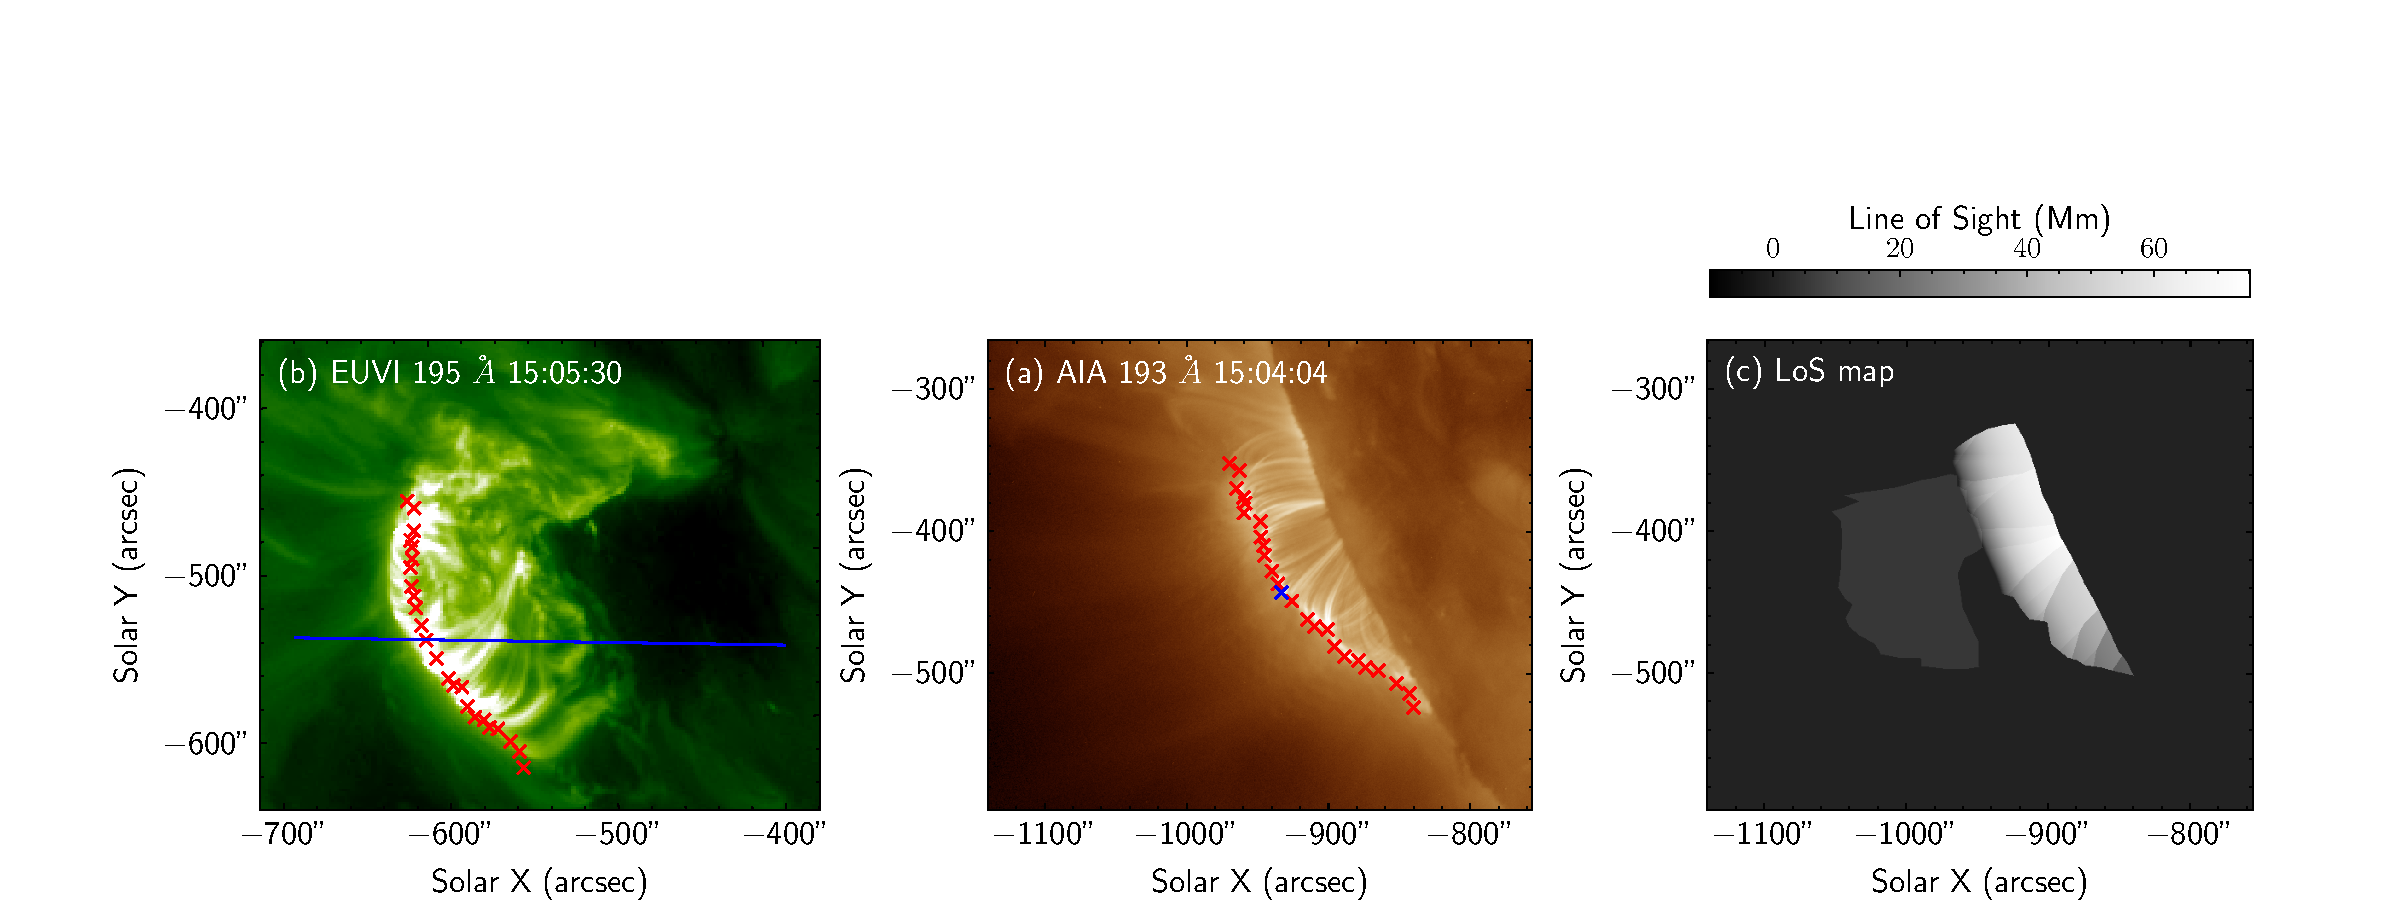
\includegraphics[width=\textwidth, trim={1cm 0cm 1cm 3cm}, clip]{paper_plot_los.pdf}
    \caption[LoS triangulation for the Nov 29th, 2020 flare]{(a) SDO/AIA 193 {\AA} observation of the Nov 29 flare in the decay phase. The red and blue crosses marks various points on the top of the arcade used to trace the looptop. The LOS goes into the page from AIA perspective. (b) {\it STEREO-A}/EUVI 195 {\AA} observation around same time. The blue solid line is the LOS from AIA perspective in panel (a) projected onto {\it STEREO-A} perspective. The red crosses mark the other red crosses from AIA perspective marked on the looptop visible from Stereo-A perspective. The line of sight of the region is shown in panel (c). The LoS is higher near the base of the loops and lower near the looptop. The fan is assumed to be constant LoS.}
    \label{fig:flare_orient2}
\end{figure*}
%%--------------

%%--------------
\begin{figure*}
    \centering
    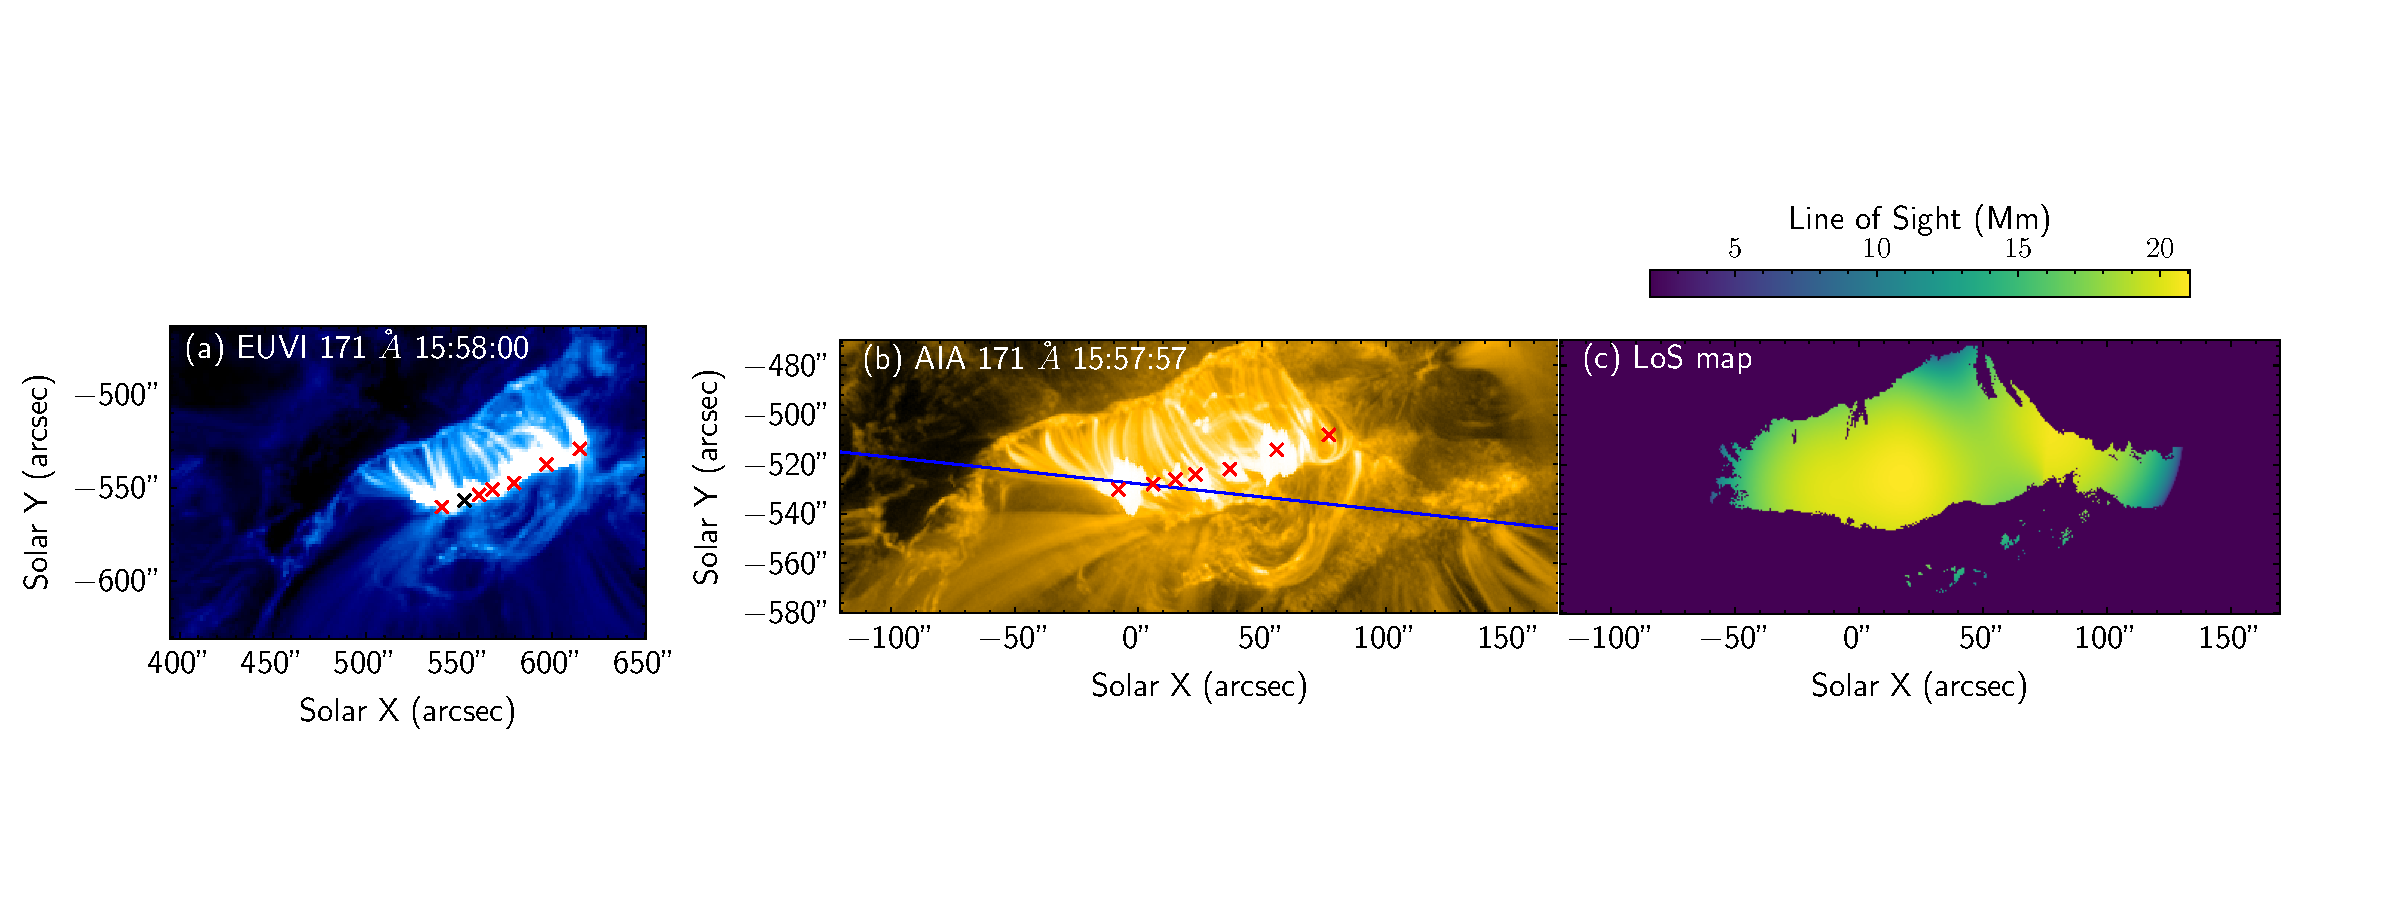
\includegraphics[width=\textwidth, trim={1cm 0cm 1cm 3cm}, clip]{paper_plot_los_2.pdf}
    \caption[LoS triangulation for the Oct 28th, 2021 flare]{(a) {\it STEREO-A}/EUVI 171 {\AA} observation of the {\bf Oct 28} flare arcade in the decay phase. The red and black cross marks a point on the top of the arcade. The line of sight (LOS) goes into the page through that point. (b) SDO/AIA 171 {\AA} observation of the flare arcade. The blue line marks the LOS through the arcade from the STEREO-A perspective projected to the AIA perspective. The red crosses mark the other red crosses from Stereo-A perspective marked on the loop top visible from AIA perspective. The line of sight of the region is shown in panel (c).}
    \label{fig:flare_orient}
\end{figure*}
%%--------------

The extent of the flare arcade is calculated by selecting pixels from the FOV which are located within an emission measure contour of 5\% of the peak emission measure value. It is possible to calculate the extent of the flare arcade from the intensity observed from any of the {\it SDO}/AIA or STIX imaging (for further details about the STIX imaging procedure, please refer to \cite{massa20}). However, due to the highly multi-thermal nature of the plasma, this procedure might be prone to missing significant portions of the flare arcade. The emission measure inferred from the DEM, on the other hand, reflects the density of the plasma in the entirety of the concerned temperature range of $5<\log\,(T)<7.4$. Therefore we find that, a 5\% contour of peak emission measure gives a better estimate of the extent of flare arcade. Outside of the flare arcade, we assume a LOS~$\sim$~2 Mm (the average thickness of chromosphere). 

%%%%%%%%%%%%%%%%%%%%%%%%%%%%%%%%%%%%%%%%%%%%%%%%%%%%
\subsection{Energy in the non-thermal electrons}\label{sec:non-therm}
%%%%%%%%%%%%%%%%%%%%%%%%%%%%%%%%%%%%%%%%%%%%%%%%%%%%

We estimate the energy in the non-thermal electrons for the 2021 Oct 28 X-class event by fitting the STIX spectra. In Fig.~\ref{fig:stix_an}.a, we plot the STIX light curve of the event in 4 to 10 keV (solid blue line), 10 to 15 keV (solid orange line), 15 to 25 keV (solid green line) and 25 to 50 keV (solid red line). The attenuator kicked in around $\sim$ 15:28 UT, which drastically cuts down the intensity to avoid saturation. The hard X-ray peak is visible in the 25 to 50 keV (solid blue line) at $\sim$ 15:28 UT. The soft X-ray peak is visible within the attenuated flux in 6 to 12 keV (solid magenta line) at $\sim$ 15:30 UT.

%%--------------
\begin{figure*}
    \centering
    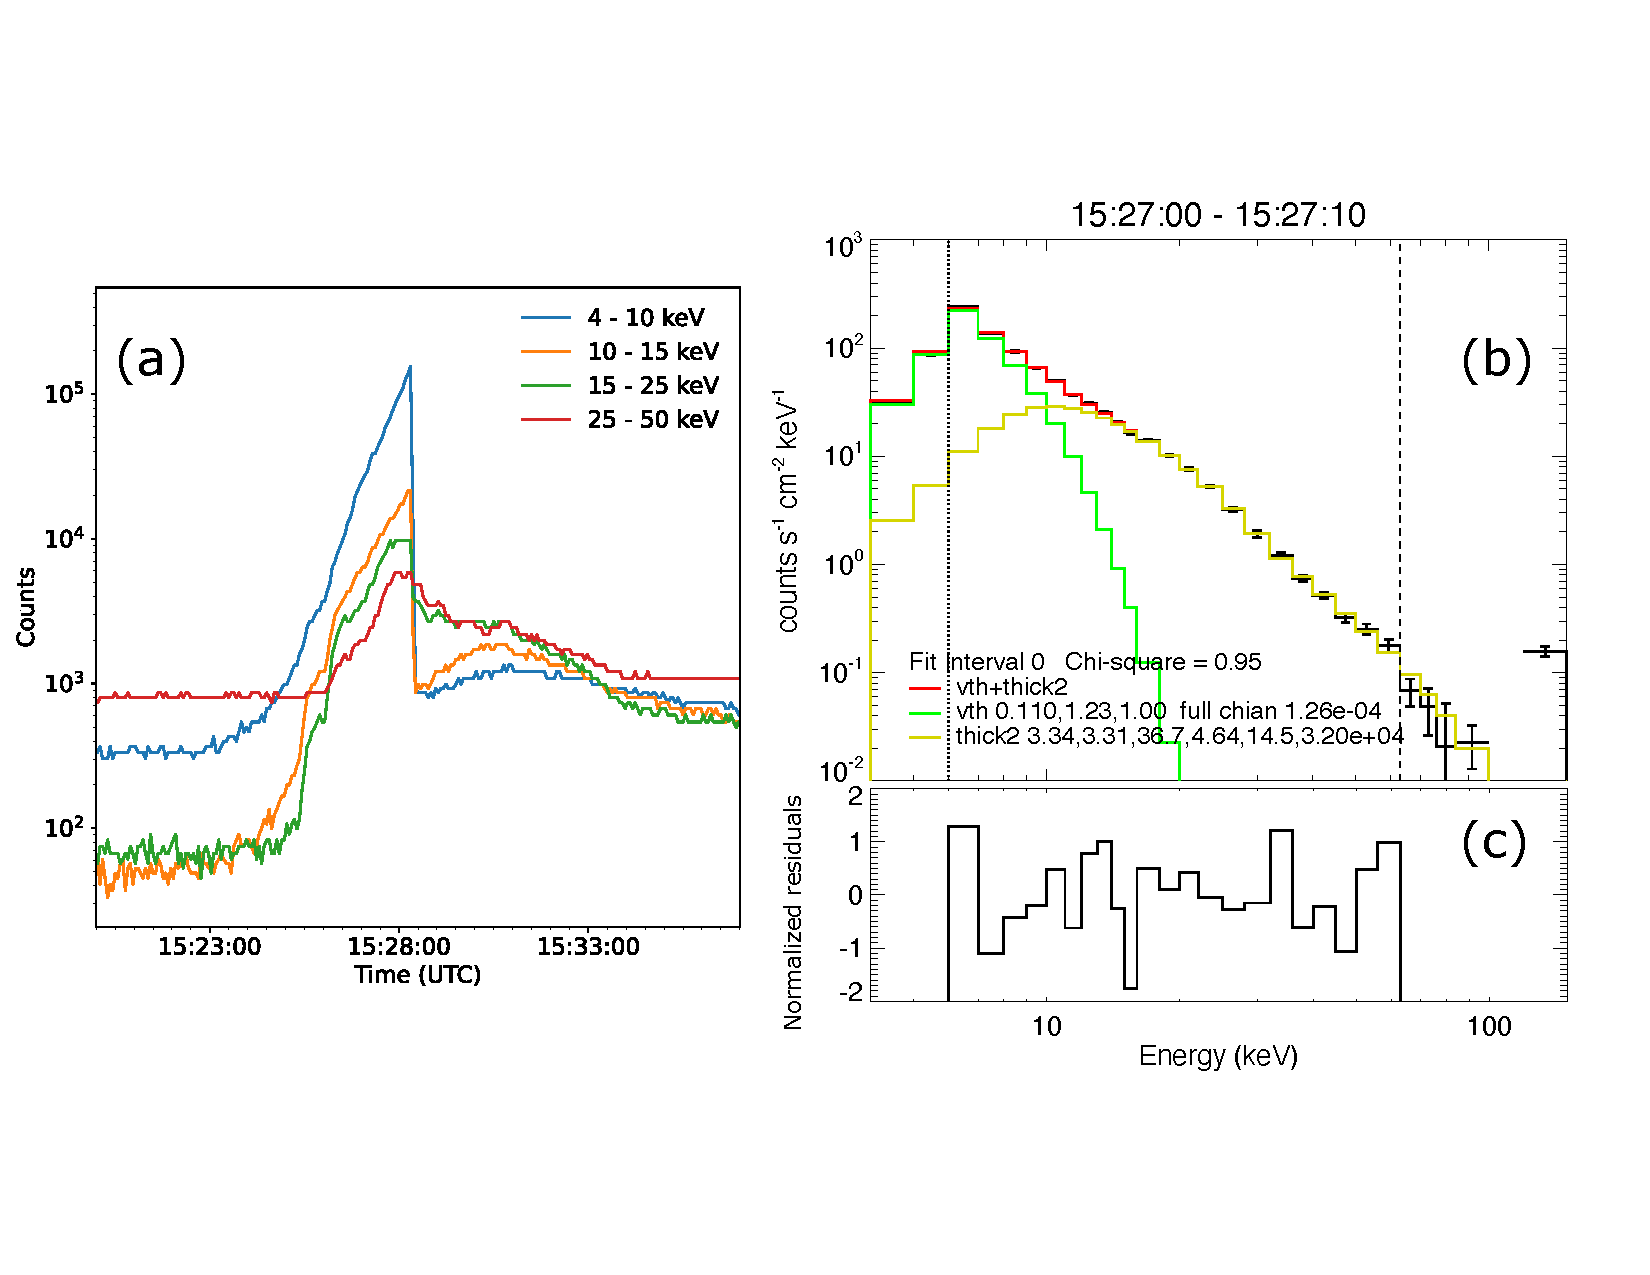
\includegraphics[trim={0cm 3cm 1.3cm 3cm}, clip, width=\textwidth]{Figures/oct_28_lc_3.pdf}
    \caption[STIX light curve and spectra fit for the 2021 Oct 28 flare]{Panel a: STIX light curve of the 2021 Oct 28 X-class event in different energy bands as labeled. Panel b: STIX spectra integrated between 15:27:00{--}15:27:10~UT during impulsive phase, fitted with `\textit{thcik2}' (solid yellow), `\textit{vth}' (solid green) and the complete fit function `\textit{vth+thick2}' (solid red line). The panel (c) shows the normalized residuals of the fit.}
    \label{fig:stix_an}
    \end{figure*}
%%--------------

We closely follow the method described in \cite{emslie12} to estimate the energy deposited by the non-thermal electrons. We fit the STIX spectra of the event averaged over several time bins during the evolution of the flare with `\textit{vth}' and `\textit{thick2}' functions available in the `\textit{OSPEX}' X-ray spectra fitting package in {\it sswidl}. We show a reference fit to the spectra obtained over a time bin $\sim$ 15:27:00-15:27:10 UT in Fig.~\ref{fig:stix_an} panel (b) with `\textit{vth}' (solid green) and `\textit{thick2}' (solid yellow). The function `\textit{vth}' is a two-component thermal function. The parameters are the emission measure and temperature of the two thermal components and the relative abundances of Iron/Nickel, Calcium, Sulfur and Silicon with respect to the coronal abundances of CHIANTI \citep{chianti1,chianti}. The `\textit{thick2}' assumes the non-thermal component to be bremsstrahlung from energetic electrons with an injected spectrum $F_{0}(E_{0})~(e^{-}s^{-1}cm^{-2}keV^{-1})$ in the form of a broken power law:

%%--------
\begin{equation}
    F_{0}(E_{0})=A
    \begin{cases}
        0, & E_{0}<E_{min} \\
        E_{0}^{-\delta_{1}}, & E_{min} \le E_{0} < E_{b} \\
        E_{0}^{-\delta_{2}}E_{b}^{\delta_{2}-\delta_{1}}, & E_{b} \le E_{0} < E_{max} \\
        0, & E_{max} \le E_{0}
    \end{cases}
\end{equation}
%%--------

The parameters of this model spectrum, e.g., the normalization parameter A, the low- and high-energy cutoffs $E_{min}$ and $E_{max}$, break energy $E_{b}$, the power law indices $\delta_{1}$ and $\delta_{2}$ below and above the break are constrained by the fitting. We only fix the high energy cutoff at $3.2\times 10^{4}$ keV for every fit. The high energy cutoff is fixed much higher than our concerned energy range ($\sim$ O($10^{1}$ keV)), and we can safely assume that it has a negligible effect on fitting the X-ray spectra \citep{emslie12}. {\bf While this serves our purpose of quantifying the bulk non-thermal energy as a function of time, there can be finer details of the physical parameters from the "cold thick target" model that can pose non-physical conditions during the early rise phase of the flares. This can also have noticeable effect on the total thermal energy budget of the flare. To mitigate this several modifications of the cold thick target model have been proposed, e.g., local re-acceleration of electrons and ions \citep{brown09}, warm thick target model \citep{kontar15, kontar19} and injection of kappa distributed electrons instead of power law \citep{kasparova09, bataglia15, effenberger17}. We describe the physical origin of some of these models and their effects on the inferred injected electron spectra in Appendix~\ref{c:a2}. We also fit two of the modified models to the same spectra and compare the differences that arise due to that.}

The `\textit{OSPEX}' fitting is done by a forward fitting procedure. The parameters of the functions `\textit{vth}' and `\textit{thick2}' are varied to generate a photon spectrum, which is folded through the detector response matrix to produce a count rate spectrum. This count rate spectrum is used to constrain the parameters of the functions through an iterative procedure by minimizing the $\chi^{2}$ between the calculated and measured count rate spectrum. We provide the fitted temperature and the EM of the hotter thermal component in Tab.~\ref{tab:tab1} during various phases of the flare. The temperatures listed in Tab.~\ref{tab:tab1} is lower than the upper limit of the temperature range used ($5.0 \geq \log\,T \leq 7.4)$ %($log(T_{max})~=~7.4$ and $log(T_{min})~=~5$) 
to calculate the EM and DEM weighted temperature in \S\ref{sec:therm}.

%%%%%%%%%%%
\begin{table}
    \centering
    \resizebox{0.9\textwidth}{!}{%
    \begin{tabular}{|cl||c|c|}
    \hline
         &  & log(T) & EM \\ 
         & \hspace{-1cm}Time (UT) & of thermal component & ($cm^{-3}$) \\
    \hline
        Impulsive phase & \hspace{1.5cm}15:26 & 7.098 & $10^{48}$\\
        HXR peak & $\sim$ 15:27:20 - 15:28:20 & 7.19 & $3\times 10^{48}$\\
        Right after SXR peak & $\sim$ 15:35:39 - 15:36:34 & 6.88 & $4.1\times 10^{49}$\\
        Into the decay phase & \hspace{0.9cm}14:48:20 & 6.5 & $2\times 10^{49}$\\
        \hline
    \end{tabular}}
    \caption{Fitted temperature of the hotter component of the thermal plasma during various stages of the flare.}
    \label{tab:tab1}
\end{table}
%%%%%%%%%%%

The non-thermal energy in the electrons ($U_{e}$) at any instant $t=t'$ can be estimated by integrating the best-fit electron energy spectrum via: $$U_{e}(t=t')~=~\Delta t\int_{E_{min}}^{E_{max}}~F_{0}(E_{0})(t=t')dE_{0}$$ where the electron energy distribution in constrained by fitting the count spectra for the time interval $t'-\Delta t/2 \le t \le t'+\Delta t/2$. The cumulative energy deposited into the foot point over time by the non-thermal electrons is a good indicator for the source of the thermal energy of the plasma. We add the energy deposited at the foot points by the non-thermal electrons from every time bin, to estimate the cumulative energy deposited by the non-thermal electrons up until that instant: $$U^{cumulative}_{e}(t)~=~\sum_{t'=t_{0}}^{t}U_{e}(t')$$.

%%%%%%%%%%%%%%%%%%%%%%%%%%%%%%%%%%%%%%%%%%%%%
\section{Results}\label{res}
%%%%%%%%%%%%%%%%%%%%%%%%%%%%%%%%%%%%%%%%%%%%%   

We plot the estimated thermal and non-thermal energy as a function of time in Fig.~\ref{fig:eneg}.a. The black solid curve with crosses and red solid curve shows the evolution of thermal energy estimated using DEM and temperature from AIA and GOES light curves, respectively. Note that, since GOES does not provide any spatial information, in order to obtain the effective volume we first estimate the loop length using RTV scaling \citep{rtv78,serio91}. For this purpose we use the EM obtained from GOES and assume a volume filling factor of 1. Note that since the RTV scaling implicitly assumes that the flare arcade is in mechanical equilibrium, the effective volume estimated using this method will only be applicable during the decay phase of the flare. Since, the assumption of filling factor to be 1 may also be susceptible to uncertainties, we also compute and plot the thermal energy evolution curve using \textit{f}~=~0.4 (green solid line with triangles) and \textit{f}~=~0.2 (blue solid line with squares). We also over plot, the thermal energy that is computed using the EM and temperature obtained from GOES but the volumed inferred from STIX soft X-ray contours, under the assumption that $V\sim A^{\frac{3}{2}}$ (purple dotted line).

%%###########%%
\begin{figure}[ht!]
    \centering
    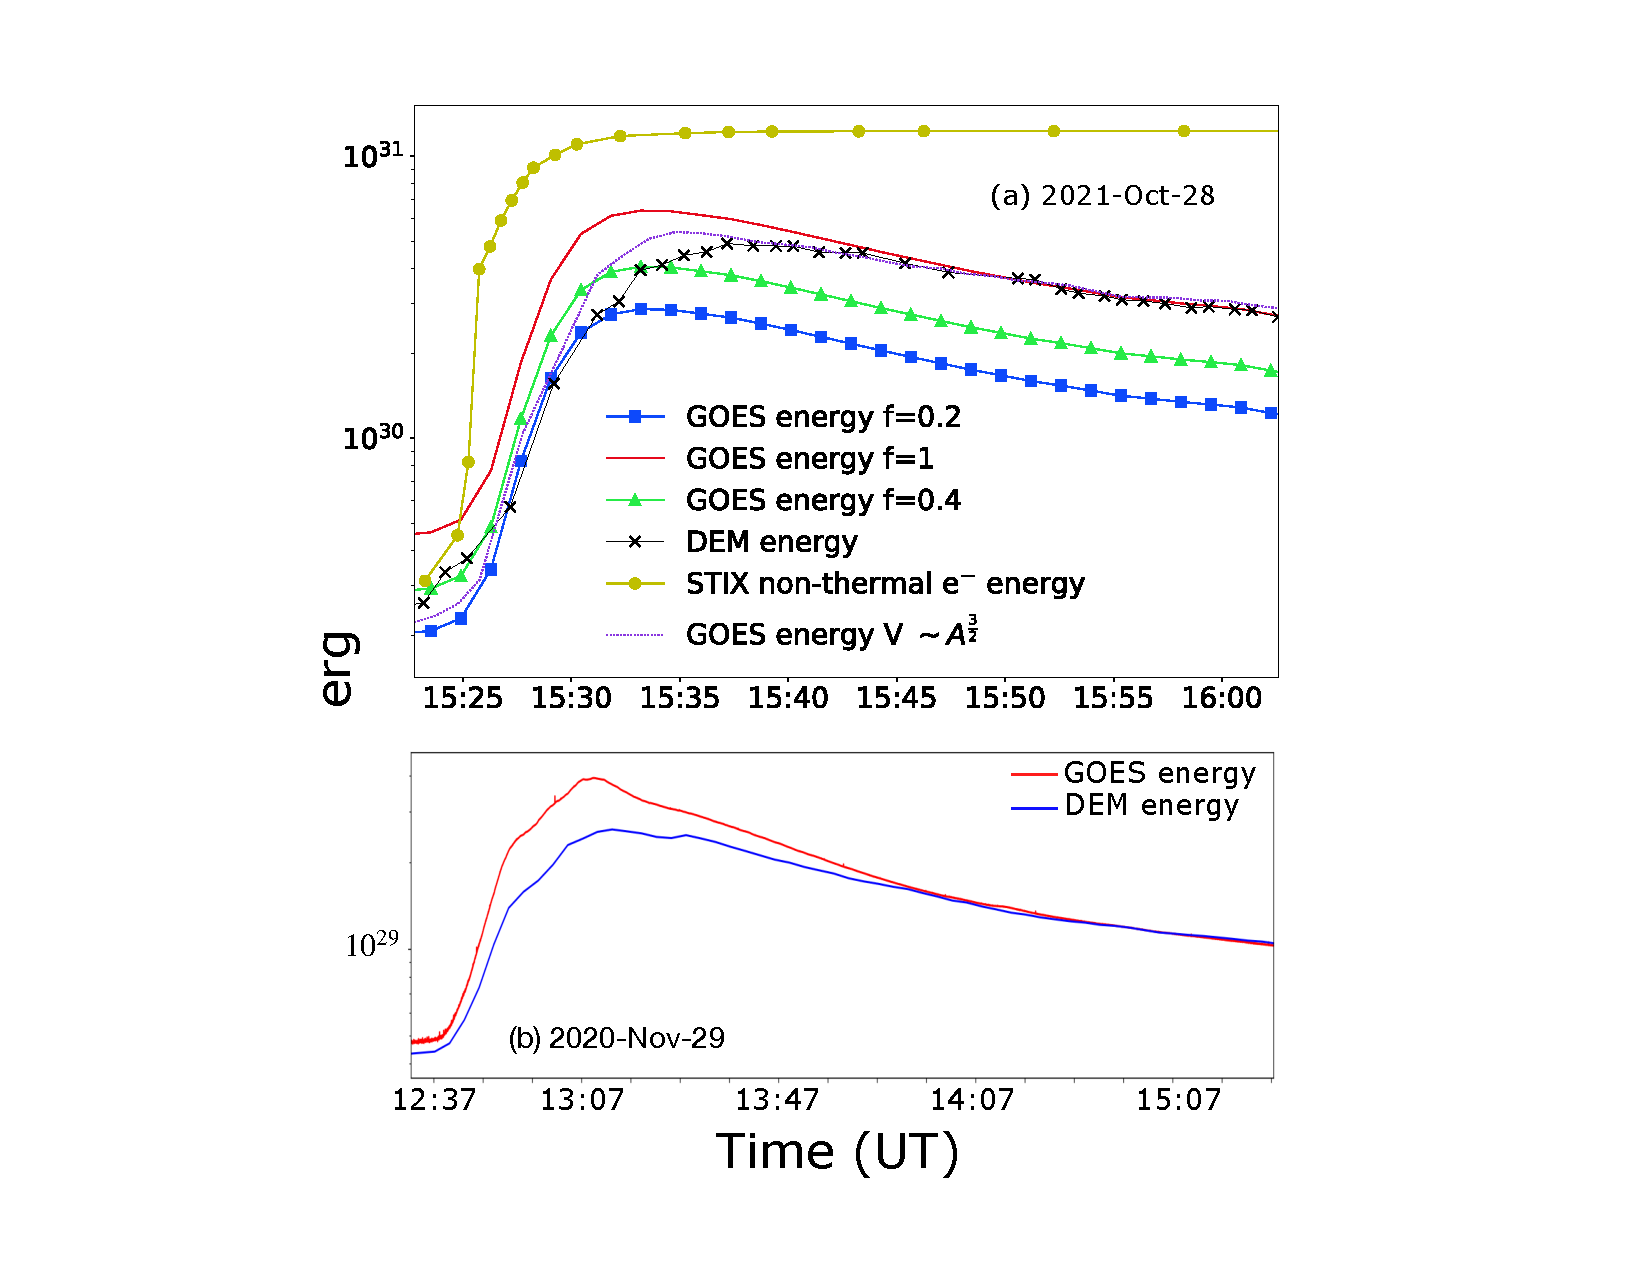
\includegraphics[trim={4cm 1cm 4cm 1cm},clip,width=0.8\textwidth]{flare_eneg.pdf}
    \caption[Temporal evolution of the thermal and non-thermal energy for both flares.]{Panel (a): Temporal evolution of thermal energy for the 2021 Oct 28 flare as measured using GOES light-curve using the effective volume and a filling factor \textit{f}~=~1 (solid red), \textit{f}~=~0.4 (green triangles), \textit{f}~=~0.2 (blue squares), thermal energy calculated from GOES light curve, but the volume inferred from the area of the of the flaring arcade with STIX SXR images, under the assumption that $V\sim A^{\frac{3}{2}}$ (purple dotted), and DEM obtained from AIA observations (black crosses). We also plot the evolution of non-thermal energy as estimated from STIX (lime green circles). Panel (b): Temporal evolution of thermal for the 2020 Nov 29 flare as measured from GOES light curves with a constant effective volume (solid red) and that calculated from the DEMs inferred from the imaging and a varying volume from the imaging (solid blue).}
    \label{fig:eneg}
\end{figure}
%%###########%%

The interesting trend in Fig.~\ref{fig:eneg}.a is that the thermal energy calculated from the constrained DEMs (solid black curve with crosses) is closer to a volume filling factor \textit{f}~=~0.2 (solid blue curve with squares) in the impulsive phase, but is asymptotic with a filling factor \textit{f}~=~1 (solid red curve) during the decay phase. This result indicates that the flare loops during the impulsive phase do not fill up apparent volumes similar to those in the decay phase. The change in the effective filling factor is indicative of the sharp change in the volume during the impulsive phase.

The lime green solid line with circles in Fig.~\ref{fig:eneg}.a, shows the cumulative energy in the non-thermal electrons. This quantity is the amount of energy deposited at the flare foot points, and one of the sources of the thermal energy of the flare. The cumulative non-thermal energy of electrons $\simeq~1.2\times 10^{31}$ erg $>$ peak thermal energy calculated from the DEM estimates $\simeq~5\times 10^{30}$ erg.

For the 2020 November 29 event, the {\it STEREO-A} perspective looks down into the supra-arcade plasma sheet. Thus the LOS of this feature can not be calculated as demonstrated in Section \ref{sec:los} for the supra-arcade pixels. For the supra-arcade fan pixels in the FOV, we assume a LOS $\simeq~8~\textrm{Mm}$, as suggested in several other studies \citep[see e.g.,][]{savage10,seaton17,li18}. We use these calculated LOS maps, along with Eqn.~\ref{eq:t_eneg_1} to estimate the thermal energy as a function of time and plot it in Fig.~\ref{fig:eneg}.b. The blue solid curve shows the thermal energy calculated from the DEMs. The red solid curve shows the thermal energy calculated from the GOES light curves and the constant effective volume calculated assuming an RTV loop with a volume filling factor \textit{f}~=~1. The thermal energy estimated from the GOES observation, using the effective volume obtained from the RTV approximation is clearly an overestimate in the impulsive phase. But similar to the previous scenario, it is a good estimator of the thermal energy in the decay phase.

There have been several studies that suggest that the plasma in the fan is directly heated \citep{hanneman14,chen17,reeves17,warren18,cai22,xie23}. Unlike the flare arcade, the thermal output of the fan is not directly related to the energy deposited by the non-thermal electrons and ions at the foot point. Hence, this different mechanism should also be reflected in the time evolution of the thermal output of the fan, compared to the thermal output of the loops. Under the assumption of the LOS~$\mathrm{\sim 8~Mm}$ in the fan region, we separately calculate the contribution from the fan to the total thermal energy for the 2020 Nov 29 event.

%%###########%%
\begin{figure}[ht!]
    \centering
    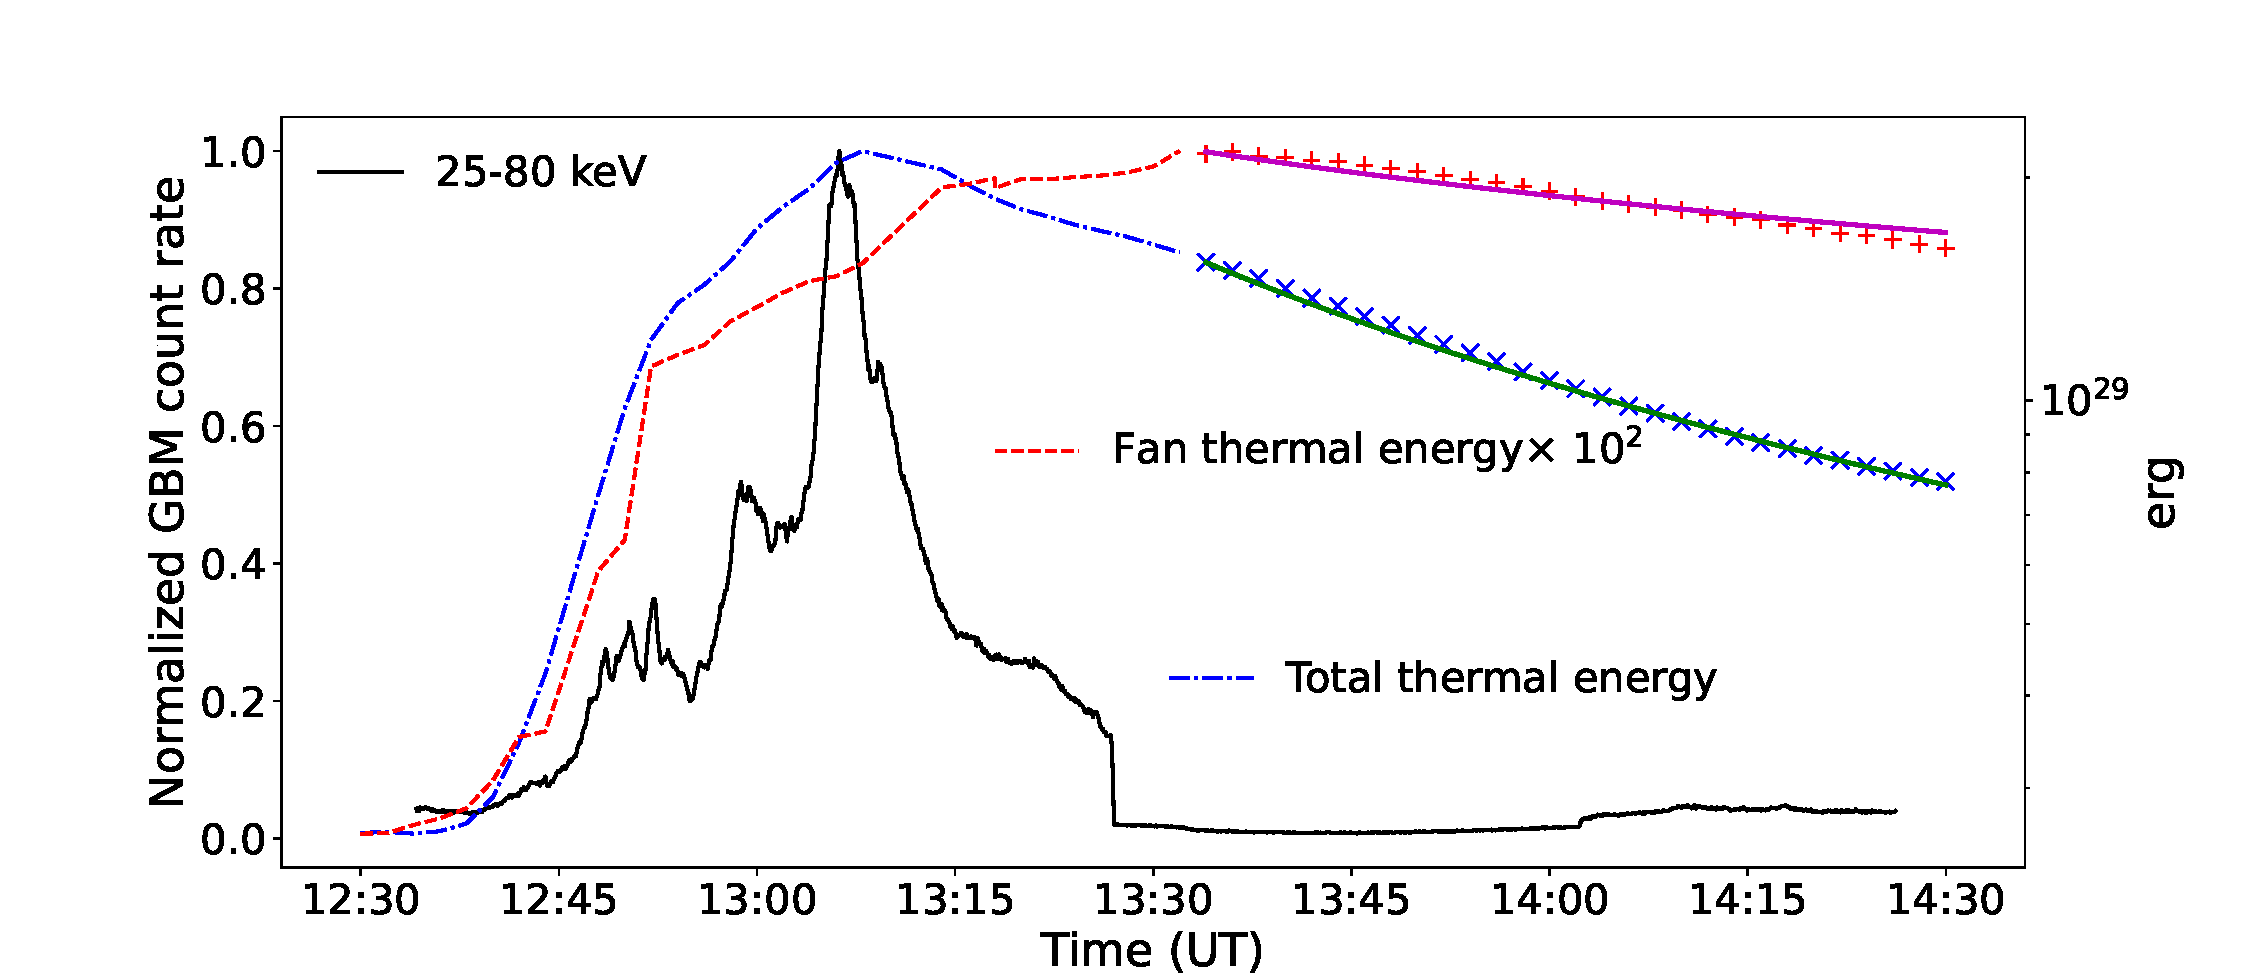
\includegraphics[trim={2cm 0cm 1cm 0cm},clip,width=0.8\textwidth]{fan_eneg.pdf}
    \caption[Calculated thermal energy for the loops and the fan for the November 29th, 2020 flare.]{Calculated thermal energy for the 2020 Nov 29 flare. The total thermal energy of the flare (blue dot-dashed) in comparison to the thermal energy from the fan (red dashed) and the Fermi hard X-ray count (black solid). The magenta and the green solid line show the fit to the thermal energy output to the fan and the loop's thermal output.}
    \label{fig:fan_eneg}
    \end{figure}
%%###########%% 

Fig.~\ref{fig:fan_eneg} shows the thermal energy of the fan as a function of time (red dashed line) in comparison to the total thermal energy of the 2020 Nov 29 event (blue dot-dashed line). The thermal energy form the fan is $\sim$ two orders of magnitude lower than the total thermal energy of the event. The thermal energy of the fan also peaks much later ($\sim$ 20 minutes) compared to the total thermal energy. After the thermal energy of the fan peaks, the thermal energy of the fan (red + sign) and the total thermal energy of the event (blue crosses) are fitted with a power law of the form $at^{-\delta}$ as a function of time. The fits are shown with magenta and green solid line for the fan and the total thermal energy, respectively. The value of the power law index are -0.95 and -1.1, respectively, for the fan and the total thermal output. The plots shows that the thermal energy of the fan decay slower compared to the total thermal output. The normalized {\it Fermi} GBM 25 {--} 80 keV count rate (black solid line) peaks at a similar time as the total thermal energy of the event. 

%%%%%%%%%%%%%%%%%%%%%%%%%%%%%%%%%%%%%%%%%%%%%
\section{Summary and Discussion}\label{sec:dis}
%%%%%%%%%%%%%%%%%%%%%%%%%%%%%%%%%%%%%%%%%%%%% 

We have used AIA, SUVI, and XRT observations to calculate DEM maps and estimate the thermal energy for two solar flares as a function of time. In addition, we have also used observations from AIA and {\it STEREO-A} to calculate the geometry of the flare loops and estimate the LOS for the AIA observations. To constrain the non-thermal energy in the 28 October, 2021 event, we have used STIX observations.  
 
Our findings suggest that a single value of volume filling factor is inadequate to describe the evolution of thermal energy throughout the duration of the flare. As such we need to estimate the volume of the flaring plasma as a function of time. In Fig.~\ref{fig:eneg}.a, the thermal energy calculated from {\it GOES} with various filling factors demonstrates this concept perfectly. During the impulsive phase, the thermal energy calculated from the DEMs is consistent with \textit{f}=0.2, and later in the decay phase, it is consistent with \textit{f}=1. This result demonstrates how the volume of the flare arcade is changing over time with respect to the volume in the decay phase. The thermal energy calculated from $V\sim A^{\frac{3}{2}}$ assumption agrees well with the thermal energy calculated from constrained DEMs in the decay phase. But it still predicts higher energy in the impulsive phase. This discrepancy signifies that the assumption of self-similar expansion may not be valid at the initial sharp rise in the impulsive phase for some flares. Our results are in line with the findings of \cite{hilarie05} (For details, please refer to Tab.5 therein and the corresponding discussion).

Our results also demonstrate the utility of estimating the volume from different vantages as a function of time. For events like the X-class event on 2021 October 28, the on-disk imaging allows the estimation of the volume from the flare ribbon area under the assumption of self-similar expansion. But for scenarios like the limb event 2020 November 29, where the flare ribbons are not visible from any imaging observation, or the visible foot point and/or visible portions of the loop are projected at a very high angle, estimating the volume of the loop by calculating the height of the loop at various points serves as an important tool in estimating the thermal energy at various phases of the flare. 

These results demonstrate that the accurate determination of volume can have significant implications for thermal energy estimates as well as partition between thermal and non-thermal energies.  While the former related to the total energetics of the flares, the later relates to the efficiency of converting the energy deposited by non-thermal electrons into the thermal energy of the ambient plasma. 


For the 2020 November 20 flare, we have also estimated the thermal energy for the fan and compared the evolution of the thermal energy of the fan with respect to the total thermal energy of the event. %We have shown that the thermal energy of the fan decays slower compared to the total thermal energy of the event. This result suggests that a fundamentally different heating mechanism is responsible for the thermal output of the fan.
In Fig.~\ref{fig:fan_eneg}, the thermal energy from the fan (red dashed line ) is $\sim$ two orders of magnitude lower than the total thermal energy of the event (blue dot-dashed line). The thermal energy also peaks much later ($\sim$ 20 minutes) compared to the total thermal energy. This result shows that the fan plasma is being heated directly by a process different from the flare arcade (e.g. SADs \citep{reeves17}, plasma flow turbulence \citep{xie23}). The fan also cools slower than the arcade, which indicates that either continuous heating is present in the fan during the decay phase of the flare or there is suppression of cooling \citep[e.g.][]{xie23}. The event had both foot points occulted from the Earth's perspective, so it is a fair assumption that most of the hard X-ray is from the loop top coronal source. This circumstance explains the near-simultaneous peak in {\it Fermi} hard X-ray (black solid line) and the thermal energy peak from the flare.

Our results exhibit the importance of different solar missions that can observe the Sun with higher spatial resolution (to resolve the finer structures better) and from various vantages (to triangulate the geometry). The ability to spatially resolve the temperature structure of the flaring plasma not only gives us a better estimation of the thermal energy, but it also allows us to spatially separate various portions of the flaring plasma (e.g. for the 2020 November 29 event, we could separate the contribution of the fan from the total thermal energy). This separation enables us to demonstrate that a different heating mechanism was at play in the fan. However, we do note that the reliability of any such estimations needs to be rigorously tested with observations of various flares from various geometric projections.